\chapter{Implementasi dan Pengujian}

Bab ini mecakup implementasi dan pengujian sistem hasil rancangan yang telah dijelaskan pada bab sebelumnya. Pada bab ini bagian implementasi tidak mencakup seluruh proses dan detail pada sistem. Detail tersebut dapat dilihat pada hasil implementasi (https://github.com/ibrohimislam/ngfilter). Sedangkan pada bab ini dijelaskan bagian menarik dari implementasi tersebut.

Pada bagian pengujian dijelaskan analisis pengujian yang memungkinkan dan alasan memilih pengujian. Pengujian yang dilakukan dengan transparent-firewall dipilih dengan alasan feasibilitas waktu yang dijelaskan pada bab ini. Kemudian dilanjutkan dengan hasil pengujian dan pembahasan.

\section{Implementasi ngfilter}

Implementasi dilakukan dengan membuat sebuah modul kernel \verb|xt_ngfilter| dan  \textit{shared library} \verb|libxt_ngfilter.so|.
Modul kernel digunakan untuk melakukan pencocokan, sedangkan \verb|libxt_ngfilter.so| berinteraksi dengan user melalui iptables.

\begin{lstlisting}
static struct xtables_match ngfilter_mt_reg = {
	.version = XTABLES_VERSION,
	.name = "ngfilter",
	.revision = 0,
	.family = NFPROTO_IPV4,
	.size = XT_ALIGN(sizeof(struct xt_ngfilter_mtinfo)),
	.userspacesize = XT_ALIGN(sizeof(struct xt_ngfilter_mtinfo)),
	.help = ngfilter_match_help,
	.init = ngfilter_match_init,
	.parse = ngfilter_match_parse,
	.final_check = ngfilter_match_check,
	.print = ngfilter_match_print,
	.save = ngfilter_match_save,
	.extra_opts = ngfilter_match_opts,
};
\end{lstlisting}

\begin{lstlisting}
static struct xt_match ngfilter_match4_reg __read_mostly = {
	.name = "ngfilter",
	.revision = 0,
	.family = NFPROTO_IPV4,
	.match = ngfilter_match,
	.checkentry = ngfilter_match_check,
	.destroy = ngfilter_match_destroy,
	.matchsize = sizeof(struct xt_ngfilter_mtinfo),
	.me = THIS_MODULE,
};
\end{lstlisting}

Instance struct \verb|xtables_match| digunakan untuk mendefinisikan modul match yang diimplementasi di userspace.
Property \verb|help|, \verb|init parse|, \verb|final_check|, \verb|print|, \verb|save|, dan \verb|extra_opts| merupakan \textit{function pointer} yang mengarah ke fungsi yang telah diimplementasi.

\begin{itemize}
\item \verb|ngfilter_match_init| dieksekusi saat modul di-\textit{register}.
\item \verb|ngfilter_match_exit| dieksekusi saat modul di-\textit{unregister}.
\item \verb|ngfilter_match_help| digunakan untuk menampilkan pesan bantuan ketika dipanggil dari \verb|iptables|.
\item \verb|ngfilter_match_parse| dieksekusi saat perintah dengan modul match \verb|ngfilter| ditambahkan ke rule. Fungsi ini melakukan mapping dari parameter perintah iptables ke dalam struktur data \verb|xt_ngfilter_mtinfo|.
\item \verb|ngfilter_match_check| merupakan fungsi yang dieksekusi saat melakukan validasi rule dengan menggunakan modul match \verb|ngfilter|.
\item \verb|ngfilter_match_print| merupakan fungsi untuk menampilkan rule yang sedang aktif. Fungsi ini dieksekusi ketika perintah \verb|iptables -L| dijalankan.
\item \verb|ngfilter_match_save| merupakan fungsi yang digunakan ketika perintah \verb|iptables-save| dijalankan. Fungsi ini melakukan mapping dari struktur data ke parameter perintah iptables sehingga dapat disimpan.
\end{itemize}

Berikut adalah definisi struct yang digunakan untuk berkomunikasi antara user-space dan kernel module.

\begin{lstlisting}
#define MAX_PATTERN_LENGTH 256
struct xt_ngfilter_mtinfo {
	unsigned char pattern[MAX_PATTERN_LENGTH];
	unsigned char smb_command;
	__u8 flags;
};
\end{lstlisting}

\section{Implementasi Rule iptables}

Penangkalan paket malicious dapat dilakukan dengan menggunakan rule iptables dengan menambahkan modul yang terlah diimplementasi sesuai desain pada subbab III.6. Penangkalan paket \textit{malicious} dapat ditangani dengan menggunakan modul \verb|ndpi-netfilter| dan modul \verb|ngfilter| dengan rule iptables sebagai berikut:

\begin{lstlisting}
-t mangle -A PREROUTING -j CONNMARK --restore-mark
-t mangle -A POSTROUTING -j CONNMARK --save-mark
-A FORWARD -m ndpi --smb  -m ngfilter --smb-command 0a -j MARK --set-xmark 0x1/0xffffffff
-A FORWARD -m mark --mark 0x1 -j LOG --log-prefix "MARK 1: "
-A FORWARD -m mark --mark 0x1 -m ngfilter --smb-command 33 -j MARK --set-xmark 0x2/0xffffffff
-A FORWARD -m mark --mark 0x2 -j LOG --log-prefix "MARK 2: "
-A FORWARD -m mark --mark 0x2 -j DROP
\end{lstlisting} 

\section{Analisis Pengujian}

Berkaitan dengan cara penyebaran worm, terdapat 2 penempatan firewall yang perlu diperhatikan, yaitu firewall di antara subnet dan firewall dalam sebuah subnet. Penempatan ini berbeda perilakunya jika dilihat dari sifat worm yang melakukan local-scanning dan random-scanning. Kedia jenis penempatan dapat mendeteksi random-scanning namun tidak dapat mendeteksi local-scanning.

Firewall di antara subnet merupakan firewall yang bekerja sebagai router (layer TCP/IP) sekaligus melakukan filtering. Firewall umumnya ditemukan dengan penempatan ini. Firewall dengan penempatan ini dapat melakukan penjagaan lalu lintas antar subnet. Namun tidak dapat menjamin pengamanan antar host dalam subnet tersebut. Sehingga, jika terdapat host yang terinfeksi worm dan melakukan subnet-local-scanning firewall tidak dapat mendeteksi aktivitas tersebut.

Cara penempatan firewall pada sebuah subnet dapat melakukan penjagaan pada sekelompok host dan memisahkannya dari host yang lain dalam sebuah subnet. Firewall dengan penempatan ini umumnya disebut transparent firewall. Penempatan ini dapat mendetaksi aktivitas subnet-local-scanning jika melintasi firewall.

Karena dibatasi waktu, pengujian dengan menempatkan firewall di antara subnet tidak dapat dilakukan karena memerlukan sumber daya dan waktu yang tidak dapat dipenuhi.  Keadaan tersebut dapat diperkirakan seperti persamaan \ref{eqn:prob_one}-\ref{eqn:expected_time}.

Jika seperti pada persamaan \ref{eqn:prob_one}, $P(1)$ adalah kemungkinan kemunculan sebuah ip maka $P(n)$ (persamaan \ref{eqn:prob_n}) merupakan kemungkinan muncul salah satu dari n ip. Sehingga diperlukan ekspektasi percobaan yang diperlukan untuk menemukan ip adalah $E(n)$ kali percobaan (persamaan \ref{eqn:expectation_n}). Jika kecepatan scanning adalah $v(1)$ dan kecepatan m buah host adalah $v(m)$, $v(m)$ dapat didekati dengan m kali $v(1)$ (persamaan \ref{eqn:velocity_m}). Jika perkiraan waktu yang dibutuhkan untuk menemukan 1 dari n ip, dengan m host yang melakukan percobaan dengan kecepatan $v(1)$ adalah $t(n,m)$, maka waktu yang dibutuhkan adalah jumlah percobaan yang diperlukan dibagi dengan kecepatan.

Dari pengamatan yang dilakukan kecepatan scanning secara random adalah 1064 ip per menit. Maka dengan persamaan \ref{eqn:expected_time} dengan 32 host terinfeksi dan 32 host target dibutuhkan 3 hari untuk mendapatkan satu serangan. Jika 1 serangan dianggap satu data maka untuk mendapatkan 10 data setidaknya diperlukan waktu 30 hari.

\begin{equation}
\label{eqn:prob_one}
P(1) = \frac{1}{2^{32}-1}
\end{equation}

\begin{equation}
\label{eqn:prob_n}
P(n) = \frac {n}{2^{32}-1}
\end{equation}

\begin{equation}
\label{eqn:expectation_n}
E(n) = \frac{1}{P(n)} = \frac{2^{32}-1}{n}
\end{equation}

\begin{equation}
\label{eqn:velocity_m}
v(m) \approx m \times v(1)
\end{equation}

\begin{equation}
\label{eqn:expected_time}
t(n,m) = \frac{E(n)}{v(m)} \approx \frac{2^{32}-1}{n \times m \times v}
\end{equation}

\section{Skenario Pengujian}

Pengujian dilakukan menggunakan membandingkan hasil percobaan kontrol dengan percobaan yang menggunakan firewall hasil implementasi. Percobaan dilakukan pada sebuah hypervisor yang memiliki spesifikasi pada tabel \ref{table:hypervisor_specification}. Percobaan ini dilakukan dengan menggunakan 10 virtual machine yang tidak terinfeksi, 1 virtual machine yang telah terinfeksi dan 1 firewall.

\begin{table}[H]
	\caption{Spesifikasi hypervisor yang digunakan untuk melakukan pengujian}
	\label{table:hypervisor_specification}
	\begin{tabularx}{\textwidth}{|l|X|}
		\hline
		\textbf{Spesifikasi} & \textbf{Spesifikasi yang digunakan} \\ \hline
		\textit{Processor} & Intel(R) Xeon(R) CPU E5-2620 0 @ 2.00GHz \\ \hline 
		\textit{Virtualization Infrastructure} & Qemu/KVM \\ \hline
		Linux & Linux 3.10.0-862.11.6.el7.x86\_64 \#1 SMP Tue Aug 14 21:49:04 UTC 2018 x86\_64 x86\_64 x86\_64 GNU/Linux \\ \hline
	\end{tabularx}
\end{table}


Percobaan dilakukan dengan memisahkan sebuah subnet 192.168.1.0/24 menjadi dua bagian,\textit{internal\_network} dan \textit{external\_network} seperti pada gambar \ref{fig:validation_scenario}. Kedua bagian tersebut kemudian dihubungkan dengan sebuah transparent firewall. Kemudian masing-masing bagian ditempatkan 5 host. \textit{external\_network} ditempatkan 5 host untuk menunjukan bahwa wannacry dapat menginfeksi host-host yang berada pada jaringan yang sama. 

Pecobaan kontrol dan percobaan firewall hasil implementasi akan memperlakukan \textit{internal\_network} dengan berbeda. Jika pada percobaan kontrol, firewall tidak menerapkan rule sama sekali pada chain FORWARD. Sedangkan pada percobaan firewall hasil implementasi akan menerapkan rule hasil implementasi. Sehingga hasil percobaan dapat menunjukan bagaimana perilaku malware akibat rule yang diterapkan.

Untuk mendapatkan data perilaku host-host baik pada \textit{internal\_network} maupun \textit{external\_network} pada firewall dilakukan \textit{packet capture}. Packet capture tersebut diharapkan dapat menjelaskan keadaan network external dan network internal. Keadaan penting yang perlu dilakukan pengamatan adalah kapan sebuah host terinfeksi. Dengan menggunakan definisi host terinfeksi yang telah dijelaskan sebelumnya, seharusnya dapat dideteksi ketika sebuah host mulai melakukan \textit{local-scanning}.

Seluruh proses pengambilan data menggunakan script otomasi yang dijelaskan pada lampiran A. Masing-masing percobaan dilakukan 30 menit dengan menempatkan sebuah host terinfeksi pada \textit{external\_network} pada detik ke 30. Kemudian setelah 30 menit \textit{packet capture} dihentikan dan seluruh host diatur ulang dengan melakukan cloning host yang telah disediakan.

\begin{figure}[H]
	\centering
	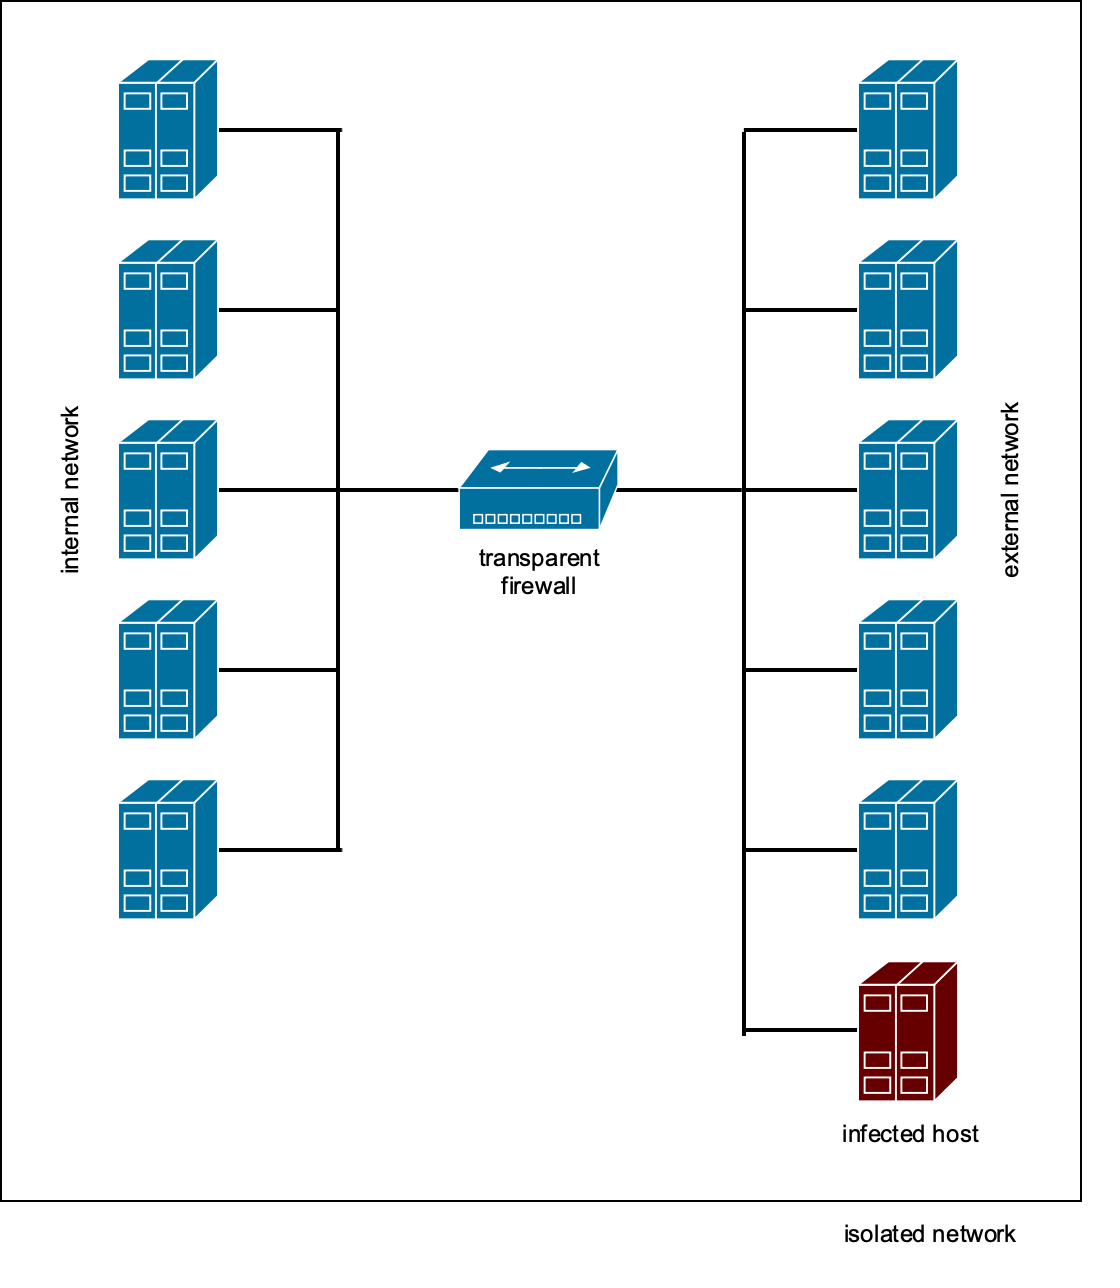
\includegraphics[width=200px]{resources/skenario_pengujian.png}
	\caption{Susunan jaringan skenario pengujian}
	\label{fig:validation_scenario}
\end{figure}

\section{Hasil Pengujian}

Data dari hasil percobaan berbentuk file pcap (\textit{packet capture}) dilakukan pengolahan untuk mendapatkan perkiraan waktu host terinfeksi. Hasil pengolahan data dapat dilihat di Lampiran B berisi data perkiraan waktu host terinfeksi. Kemudian data tersebut diakumulasikan untuk setiap percobaan untuk mendapatkan data pada suatu waktu telah ada berapa host terinfeksi.

\begin{figure}[H]
	\centering
	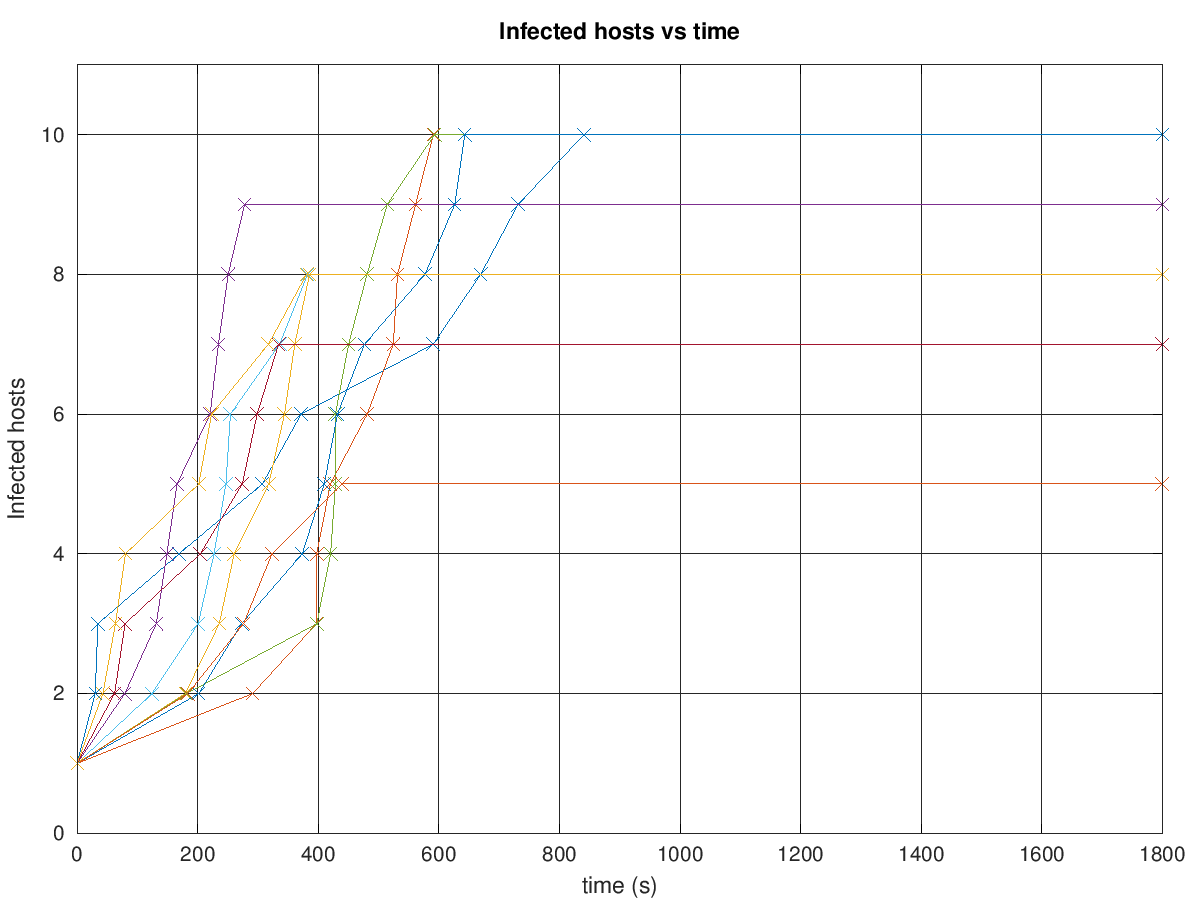
\includegraphics[width=\textwidth]{resources/infection_control_over_time.png}
	\caption{Grafik host terinfeksi terhadap waktu (percobaan kontrol)}
	\label{fig:infection_control_over_time}
\end{figure}

Grafik akumulasi host terinfeksi pada percobaan kontrol dapat dilihat pada gambar \ref{fig:infection_control_over_time}. Grafik tersebut berisi 10 data percobaan kontrol. Dari 10 percobaan tersebut dapat diperkirakan setelah 900 detik sudah terdapat lebih dari 5 host terinfeksi baik dari \textit{internal\_network} maupun \textit{external\_network}.

\begin{table}[H]
	\caption{Akumulasi detik ke-1800 host terinfeksi (percobaan kontrol)}
	\label{table:1800s_all_network_control}
	\begin{center}
		\begin{tabularx}{300px}{|X|r|}
			\hline
			\multicolumn{1}{|l}{\textbf{Jumlah host terinfeksi}} & \multicolumn{1}{|l|}{\textbf{teramati}} \\ \hline
			5 & 1 percobaan\\ \hline
			7 & 1 percobaan\\ \hline
			8 & 3 percobaan\\ \hline
			9 & 1 percobaan\\ \hline
			10 & 4 percobaan\\ \hline
		\end{tabularx}
	\end{center}
\end{table}

\begin{table}[H]
	\caption{Akumulasi detik ke-1800 host \textit{internal\_network} terinfeksi (percobaan kontrol)}
	\label{table:1800s_internal_network_control}
	\begin{center}
		\begin{tabularx}{300px}{|X|r|}
			\hline
			\multicolumn{1}{|l}{\textbf{Jumlah host \textit{internal\_network} terinfeksi}} & \multicolumn{1}{|l|}{\textbf{teramati}} \\ \hline
			2 & 1 percobaan\\ \hline
			3 & 1 percobaan\\ \hline
			4 & 4 percobaan\\ \hline
			5 & 4 percobaan\\ \hline
		\end{tabularx}
	\end{center}
\end{table}

Pada tabel \ref{table:1800s_all_network_control} dapat dilihat persebaran hasil pengamatan host terinfeksi pada \textit{internal\_network} maupun \textit{external\_network}. Sedangkan pada tabel \ref{table:1800s_internal_network_control} dapat dilihat persebaran pengamatan host terinfeksi pada \textit{internal\_network}. Kedua distribusi ini dapat menggambarkan perilaku infeksi WannaCry.

\begin{table}[H]
	\caption{Akumulasi detik ke-1800 host terinfeksi (percobaan firewall implementasi)}
	\label{table:1800s_all_network_firewalled}
	\begin{center}
		\begin{tabularx}{300px}{|X|r|}
			\hline
			\multicolumn{1}{|l}{\textbf{Jumlah host terinfeksi}} & \multicolumn{1}{|l|}{\textbf{teramati}} \\ \hline
			1 & 40 percobaan\\ \hline
			2 & 15 percobaan\\ \hline
			3 & 16 percobaan\\ \hline
			4 & 3 percobaan\\ \hline
			5 & 8 percobaan\\ \hline
			4 & 1 percobaan\\ \hline
		\end{tabularx}
	\end{center}
\end{table}

\begin{figure}[H]
	\centering
	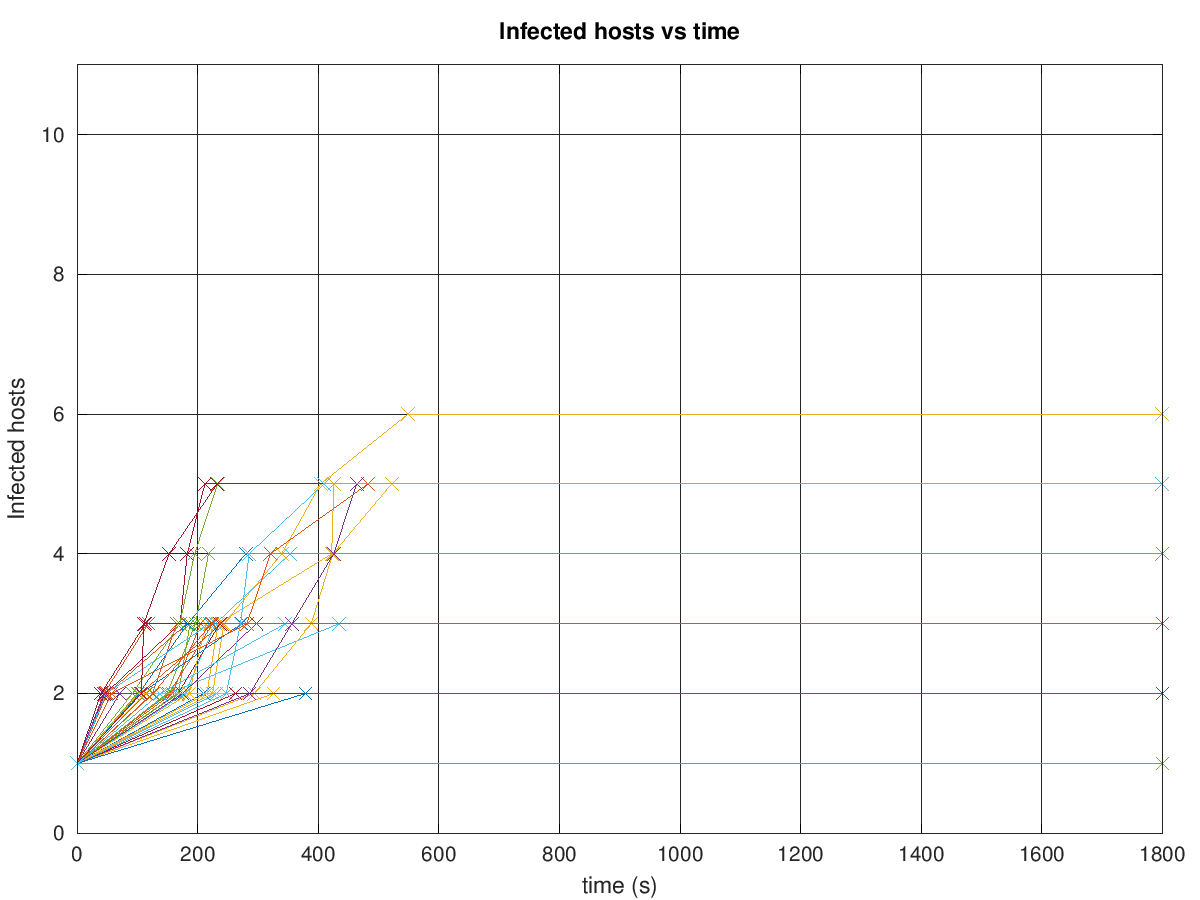
\includegraphics[width=\textwidth]{resources/infection_control_over_time_firewalled.png}
	\caption{Grafik host terinfeksi terhadap waktu (percobaan implementasi firewall)}
	\label{fig:infection_control_over_time_firewalled}
\end{figure}

Grafik akumulasi host teinfeksi pada percobaan implementasi firewall dapat dilihat pada gambar \ref{fig:infection_control_over_time_firewalled}. Persebaran pengamatan host terinfeksi pada keseluruhan network dapat dilihat pada tabel \ref{table:1800s_all_network_firewalled}. Dari 83 percobaan tidak diamati infeksi terjadi pada \textit{internal\_network}.

\section{Pembahasan}

Pada subbab ini dijelaskan bagaimana tujuan telah dicapai dari hasil pengujian yang telah dilakukan. Tujuan pada bab I berhasil dilakukan berdasarkan ...

